%\documentclass[t,mathserif,11pt,handout,usenames,dvipsnames]{beamer}
\documentclass[t,mathserif,11pt,usenames,dvipsnames]{beamer}
%\documentclass[t,mathserif,11pt]{beamer} 
%\usetheme{Berlin}
\usecolortheme{seahorse}
%\usetheme{CambridgeUS}
%\usecolortheme{rose}
%\usecolortheme{dolphin}

%\usefonttheme[onlymath]{serif}

\setbeamertemplate{itemize items}[square]
\setbeamertemplate{itemize subitem}[circle]
\setbeamertemplate{itemize subsubitem}[triangle]

\setbeamertemplate{enumerate items}[default]




\usepackage{verbatim}
%\usepackage{multirow}
\usepackage[normalem]{ulem}

%\newcommand\hmmax{0}
\usepackage{hyperref}
%\usepackage[abbrev]{amsrefs}

%\usepackage{bbold}
%\usepackage{bbm}
%\def\mathbb{\mathbbm}
\usepackage{amssymb}
\usepackage{amsmath}
%\usepackage{unicode-math}
%\usepackage{amsthm}
\usepackage{graphicx}
\usepackage{braket}
%\usepackage{paralist}
%\usepackage{rotating}
%\usepackage{arydshln}

%\usepackage{color}
\usepackage{xcolor}
%\usepackage[all,color]{xy}
%\UseCrayolaColors

%\usepackage{mathabx}
\usepackage{mathrsfs}
%\usepackage{MnSymbol}
%\usepackage{mathbbol}
%\usepackage{psnfss}



\usepackage{youngtab}
\Yautoscale1
\Yvcentermath1

\usepackage[centertableaux,smalltableaux]{ytableau}

%\usepackage{cleveref}

\theoremstyle{plain}
\newtheorem{thm}{Theorem}
\newtheorem{claim}{Claim}
\newtheorem{conj}{Conjecture}

%\newtheorem{lemA}[thmA]{Lemma}
%\newtheorem{propA}[thmA]{Proposition}
%\newtheorem{corA}[thmA]{Corollary}
%\newtheorem{thm}[subsection]{Theorem}
%\newtheorem{lemma}{Lemma}
\newtheorem{prop}{Proposition}
\newtheorem{cor}{Corollary}
%\newtheorem*{prop*}{Proposition}

\theoremstyle{definition}
\newtheorem{defn}{Definition}



\definecolor{refkey}{gray}{.3}
\definecolor{labelkey}{gray}{.3}


% \def\cone{\ding{172}}
% \def\ctwo{\ding{173}}
% \def\cthree{\ding{174}}
% \def\cfour{\ding{175}}
% \def\cfive{\ding{176}}



\newcommand{\mjjc}[1]{\marginpar{\color{green}\tiny #1 \mbox{--ma}}}


\newcommand{\rk}{\mathrm{rk}}
\newcommand{\cqq}{\mathscr{D}}
\newcommand{\Sym}{\mathrm{Sym}}
\newcommand{\rSp}{\mathrm{Sp}}
\newcommand{\rsym}{\mathrm{sym}}
\newcommand{\rO}{\mathrm{O}}
\newcommand{\SO}{\mathrm{SO}}
\newcommand{\rskew}{\mathrm{skew}}
\newcommand{\fraksp}{\mathfrak{sp}}
\newcommand{\frakso}{\mathfrak{so}}
\newcommand{\frakm}{\mathfrak{m}}
\newcommand{\frakp}{\mathfrak{p}}
\newcommand{\pr}{\mathrm{pr}}
\newcommand{\rhopst}{\rho'^*}
\newcommand{\Rad}{\mathrm{Rad}}
\newcommand{\Res}{\mathrm{Res}}
\newcommand{\Hol}{\mathrm{Hol}}
\newcommand{\AC}{\mathrm{AC}}
\newcommand{\AV}{\mathrm{AV}}
\newcommand{\VC}{\mathrm{V}_\bC}
\newcommand{\bfv}{\mathbf{v}}
\newcommand{\depth}{\mathrm{depth}}
\newcommand{\wtM}{\widetilde{M}}
\newcommand{\wtMone}{{\widetilde{M}^{(1,1)}}}

\newcommand{\nullpp}{N(\fpp'^*)}
\newcommand{\nullp}{N(\fpp^*)}
\newcommand{\Aut}{\mathrm{Aut}}



\newcommand{\bfone}{\mathbf{1}}
\newcommand{\bbone}{\mathbb{1}}




\newcommand{\sfVprime}{\mathsf{V}^\prime}
\newcommand{\sfVdprime}{\mathsf{V}^{\prime \prime}}
\newcommand{\gminusone}{\mathfrak{g}_{-\frac{1}{m}}}

\newcommand{\eva}{\mathrm{eva}}

\newcommand\iso{\xrightarrow{
\,\smash{\raisebox{-0.65ex}{\ensuremath{\scriptstyle\sim}}}\,}}

\def\tmu{\tilde{\mu}}

\def\tr{\mathrm{tr}}
\def\trD{{\tr_{D/F}}}
\def\trF{{\tr_F}}

\def\Ueven{{U_{\rm{even}}}}
\def\Uodd{{U_{\rm{odd}}}}
\def\ttau{\tilde{\tau}}
\def\Wcp{W}
\def\Kur{{K^{\mathrm{u}}}}


\providecommand{\bcN}{{\overline{\cN}}}
\providecommand{\bcO}{{\overline{\cO}}}

\def\Mpii{M'^{(1,1)}}
\def\Mptz{M'^{(2,0)}}
\def\Mpzt{M'^{(0,2)}}
\def\mpii{\fmm'^{(1,1)}}
\def\mptz{\fmm'^{(2,0)}}
\def\mpzt{\fmm'^{(0,2)}}
\def\bcOp{\overline{\cO'}}

\def\frakN{\mathfrak{N}}
\def\topform{\mbox{$\bigwedge^{\! \mathrm{top} \, }$}}

\def\barxi{{\overline{\xi}}}
\def\Stab{{\rm Stab}}
\def\ad{{\rm ad}}
\def\Ad{{\rm Ad}}
\def\id{{\rm id}}
\def\sgn{{\rm sgn}}
\def\gcd{{\rm gcd}}

\makeatletter
\def\inn#1#2{\left\langle 
\def\ta{#1}\def\tb{#2}
\ifx\ta\@empty{\;} \else {\ta}\fi ,
\ifx\tb\@empty{\;} \else {\tb}\fi
\right\rangle} 
\makeatother

\def\innw#1#2{\inn{#1}{#2}_{W}}
\def\innv#1#2{\inn{#1}{#2}_{V}}
\def\innvp#1#2{\inn{#1}{#2}_{V'}}
\def\innGa#1#2{\inn{#1}{#2}_{\Gamma}}
\def\innGap#1#2{\inn{#1}{#2}_{\Gamma'}}

\def\abs#1{\left|{#1}\right|}
\def\norm#1{{\left\|{#1}\right\|}}



\def\mydefhat#1{\expandafter\def\csname hat#1\endcsname{\hat{#1}}}
\def\mydefwh#1{\expandafter\def\csname wh#1\endcsname{\widehat{#1}}}
\def\mydeft#1{\expandafter\def\csname t#1\endcsname{\tilde{#1}}}
\def\mydefr#1{\expandafter\def\csname r#1\endcsname{\mathrm{#1}}}
\def\mydefb#1{\expandafter\def\csname b#1\endcsname{\mathbb{#1}}}
\def\mydefwt#1{\expandafter\def\csname wt#1\endcsname{\widetilde{#1}}}
\def\mydeff#1{\expandafter\def\csname f#1\endcsname{\mathfrak{#1}}}
\def\mydefbf#1{\expandafter\def\csname bf#1\endcsname{\mathbf{#1}}}
\def\mydefc#1{\expandafter\def\csname c#1\endcsname{\mathcal{#1}}}
\def\mydefsf#1{\expandafter\def\csname sf#1\endcsname{\mathsf{#1}}}
\def\mydefs#1{\expandafter\def\csname s#1\endcsname{\mathscr{#1}}}
\def\mydefcks#1{\expandafter\def\csname cks#1\endcsname{{\check{
\csname s#1\endcsname}}}}
\def\mydefck#1{\expandafter\def\csname ck#1\endcsname{{\check{
#1}}}}

\def\mydefbfdowncase#1{
\expandafter\def\csname bf#1#1\endcsname{\mathbf{#1}}
}
\def\mydefckdowncase#1{
\expandafter\def\csname ck#1#1\endcsname{\check{#1}}
}
\def\mydefrmdowncase#1{
\expandafter\def\csname r#1#1\endcsname{\mathrm{#1}}
}
\def\mydefsfdowncase#1{
\expandafter\def\csname sf#1#1\endcsname{\mathsf{#1}}
}
\def\mydeffdowncase#1{
\expandafter\def\csname f#1#1\endcsname{\mathfrak{#1}}
}

\def\doAZ#1{#1A #1B #1C #1D #1E #1F #1G #1H #1I #1J #1K #1L 
#1M #1N #1O #1P #1Q #1R #1S #1T #1U #1V #1W #1X #1Y #1Z}
\def\doaz#1{#1a #1b #1c #1d #1e #1f #1g #1h #1i #1j #1k #1l 
#1m #1n #1o #1p #1q #1r #1s #1t #1u #1v #1w #1x #1y #1z}

\doAZ{\mydefsf}
\doAZ{\mydeft}
\doAZ{\mydefwh}
\doAZ{\mydefhat}
\doAZ{\mydefr}
\doAZ{\mydefwt}
\doAZ{\mydeff}
\doAZ{\mydefb}
\doAZ{\mydefbf}
\doAZ{\mydefc}
\doAZ{\mydefs}
\doAZ{\mydefck}
\doAZ{\mydefcks}

\doaz{\mydefbfdowncase}
\doaz{\mydeffdowncase}
\doaz{\mydefrmdowncase}
\doaz{\mydefsfdowncase}
\doaz{\mydefckdowncase}




\def\wtGL{\widetilde{\GL}}
\def\wtSp{\widetilde{\rSp}}
\def\tSp{\tilde{\rSp}}


\def\trho{{\widetilde{\rho}}}
\def\tiota{{\widetilde{\iota}}}
\def\biota{{\overline{\iota}}}



\def\GL{\mathrm{GL}}
\def\wtSp{\widetilde{\mathrm{Sp}}}
\def\fsp{{\mathfrak{sp}}}
\def\fgl{{\mathfrak{gl}}}
\def\fsl{{\mathfrak{sl}}}
\DeclareMathOperator{\Wh}{Wh}
\DeclareMathOperator{\WF}{WF}

\def\Id{\mathrm{Id}}
\def\Ann{{\mathrm{Ann}\,}}
\def\Ker{{\rm Ker}\,}
\def\Lie{{\rm Lie}}
\def\Im{{\rm Im\,}}
\def\Hom{{\rm Hom}}
\def\End{{\rm End}}
\def\Mat{{\rm Mat}}
\def\Ind{{\rm Ind}}
\def\ind{{\rm ind}}
\def\Spec{{\rm Spec\,}}
\def\Supp{\mathrm{Supp}}
\def\Sym{\mathrm{Sym}}
\def\Alt{\mathrm{Alt}}
\def\Gr{\mathrm{Gr\,}}
\def\codim{\mathrm{codim}}
\def\rank{\mathrm{rank}}
\def\Gal{\mathrm{Gal}}

\def\cAV{{\cA\cV}}
\def\supp{{\rm{supp}\,}}
\def\wtMoo{{{\wtM^{(1,1)}}}}

\def\nosizesub#1#2{{{#1}_{\makebox[0pt][l]{$\scriptstyle {#2}$}}}}

% editing macros. 
\long\def\mjj#1{{{\color{magenta}#1}}}
\long\def\delete#1{}
\long\def\mjjd#1#2{{\color{blue}#1 \sout{#2}}}

\newcommand{\trivial}[2][]{\if\relax\detokenize{#1}\relax
{\green {\medskip The following is trivial. } #2}
\else 
\ifx#1h\relax  \else {\red Wrong argument!} \fi
\fi
}


\def\floor#1{{\lfloor #1 \rfloor}}
\def\ceil#1{{\lceil #1 \rceil}}
\def\foo{{\mathfrak{o}}}
\def\sV{{\mathscr{V}}}
\def\tjj{{\tilde{j}}}
\def\wtA{{\widetilde{A}}}
\def\iinn#1#2{\ll#1,#2\gg}
\def\fF{{\mathfrak{F}}}
\def\fM{{\mathfrak{M}}}
\def\Hom{{\mathrm{Hom}}}

\def\tww{{\tilde{w}}}
\def\tgg{{\tilde{g}}}
\def\hG{{\hat{G}}}
\def\LG{{{}^LG}}
\def\LN{{{}^LN}}
\def\hn{{\hat{n}}}
\def\hns{{\hat{n}_s}}
\def\hnt{{\hat{n}_t}}

\def\fppC{\fpp_\bC}
\def\fppCp{\fpp'_{\bC}}


\def\sW{{\mathscr{W}}}
\def\Stab{{\mathrm{Stab}}}
\def\Mp{{\mathrm{Mp}}}
\def\Sp{{\mathrm{Sp}}}
\def\SL{{\mathrm{SL}}}
\def\Irr{{\mathrm{Irr}}}
\def\Rep{{\mathrm{Rep}}}
\def\cX{{\mathcal{X}}}
\def\cW{{\mathcal{W}}}
\def\rG{{\mathrm{G}}}
\def\Unip{{\mathrm{Unip}}}
\def\Ch{{\mathrm{Ch}}}

\def\Xllp{{{\mathsf{X}}_{\lambda,\lambda'}}}
\def\Pil{{\pi_{\lambda,\check{\rho}}}}
\def\Pilp{{\pi'_{\lambda',\rho'}}}

\def\piSigma{{\pi_\Sigma}}
\def\piSigmap{{\pi'_{\Sigma'}}}
\def\piSigmapp{{\pi'_{\Sigma''}}}


\def\wteta{{\widetilde{\eta}}}
\def\wtpi{{\widetilde{\pi}}}
\def\tpiSigma{{\wtpi_\Sigma}}
\def\tpiSigmap{{\wtpi'_{\Sigma'}}}
\def\tpiSigmapp{{\wtpi'_{\Sigma''}}}

\def\Latto{{\mathrm{Latt^1}}}


\def\half{{\frac{1}{2}}}
\def\halfm{{\frac{m}{2}}}
\def\halfmm{{\frac{m-1}{2}}}
\def\fracmm{{\frac{1}{m}}}
\def\fracdmm{{\frac{1}{2m}}}

\def\cdt{{c}}
\def\bPsi{{\overline{\Psi}}}
\def\bpsi{{\overline{\psi}}}

\def\vG{{\overrightarrow{G}}}
\def\vrr{{\overrightarrow{r}}}
\def\vphi{{\overrightarrow{\phi}}}

\def\Cent#1#2{{\mathrm{Z}_{#1}({#2})}}

\def\bomega{{\overline{\omega}}}
\def\bomegaS{{\bomega_S}}
\def\bomegadgS{{\bomega_{\dgS}}}

%\def\cInd{{\mathrm{c-Ind}}}
\DeclareMathOperator{\cInd}{c-Ind}

\def\istar{{\filledstar}}
\def\mstar{{\medstar}}
\def\dstar{{\medstarofdavid}}

\def\skewinv{{\mathrm{skew-inv}}}
\def\btt{{\mathbbm{t}}}

\def\diagJ{{J^\triangle}}

\def\dd{{\rm{d}}}
\def\dalpha{{\dd\alpha}}
\def\dalphap{{\dd\alpha^\perp}}
\def\odalpha{\overline{\dd\alpha}}
\def\odalphap{\overline{\dd\alpha^\perp}}

\def\vol{{\mathrm{vol}}}

\def\Jump{{\mathrm{Jump}}}

\def\CO{\cO}
\def\bTheta{\overline{\Theta}}
\def\ckcO{{\check{\cO}}}
\def\ckfgg{{\check{\fgg}}}
\def\ckfgl{{\check{\fgl}}}
\def\ckGamma{{\check{\Gamma}}}
\def\ckww{{\check{w}}}
\def\ckD{{\check{D}}}

\def\sspan{{\mathrm{Span}}}

\def\dbK{{\breve{K}}}
\def\dbKp{{\dbK_+}}
\def\dbKzp{{\dbK_{0^+}}}
\def\dbpsi{{\breve{\psi}}}
\def\dbrho{{\breve{\rho}}}
\def\dbkappa{{\breve{\kappa}}}
\def\dbeta{{\breve{\eta}}}

\def\TTidx#1#2{\,{}^{#1}\hspace{-0.1em}#2}

\def\mydefTT#1#2#3{
\expandafter\def\csname ii#3{#1}\endcsname{\TTidx{i}{#2{#1}}}
\expandafter\def\csname zz#3{#1}\endcsname{\TTidx{0}{#2{#1}}}
\expandafter\def\csname ll#3{#1}\endcsname{\TTidx{l}{#2{#1}}}
\expandafter\def\csname aa#3{#1}\endcsname{\TTidx{a}{#2{#1}}}
\expandafter\def\csname bb#3{#1}\endcsname{\TTidx{b}{#2{#1}}}
\expandafter\def\csname oo#3{#1}\endcsname{\TTidx{1}{#2{#1}}}
\expandafter\def\csname ss#3{#1}\endcsname{\TTidx{\boxslash}{#2{#1}}}
\expandafter\def\csname dg#3{#1}\endcsname{\TTidx{\boxbackslash}{#2{#1}}}
}
\def\usecsname#1{\csname #1\endcsname}
\def\useLetter#1{#1}
\def\usedbletter#1{#1#1}

\def\Vp{V'}
\def\sLp{\sL'}
\def\Sigmap{\Sigma'}
\def\fggp{\fgg'}

\mydefTT{sB}{\usecsname}{\useLetter}
\mydefTT{Sigma}{\usecsname}{\useLetter}
\mydefTT{Sigmap}{\usecsname}{\useLetter}
\mydefTT{Gamma}{\usecsname}{\useLetter}
\mydefTT{Omega}{\usecsname}{\useLetter}
\mydefTT{phi}{\usecsname}{\useLetter}
\mydefTT{eta}{\usecsname}{\useLetter}
\mydefTT{kappa}{\usecsname}{\useLetter}
\mydefTT{dbkappa}{\usecsname}{\useLetter}
\mydefTT{bomega}{\usecsname}{\useLetter}
\mydefTT{rho}{\usecsname}{\useLetter}
\mydefTT{dbrho}{\usecsname}{\useLetter}
\mydefTT{bfbb}{\usecsname}{\useLetter}
\mydefTT{sL}{\usecsname}{\useLetter}
\mydefTT{sLp}{\usecsname}{\useLetter}
\mydefTT{G}{\useLetter}{\useLetter}
\mydefTT{K}{\useLetter}{\useLetter}
\mydefTT{W}{\useLetter}{\useLetter}
\mydefTT{S}{\useLetter}{\useLetter}
\mydefTT{V}{\useLetter}{\useLetter}
\mydefTT{Vp}{\usecsname}{\useLetter}
\mydefTT{dbK}{\usecsname}{\useLetter}
\mydefTT{dbG}{\usecsname}{\useLetter}
\mydefTT{End}{\usecsname}{\useLetter}

\mydefTT{x}{\useLetter}{\usedbletter}
\mydefTT{v}{\useLetter}{\usedbletter}
\mydefTT{w}{\useLetter}{\usedbletter}
\mydefTT{fgg}{\usecsname}{\useLetter}
\mydefTT{fggp}{\usecsname}{\useLetter}


\def\zzll{\ell}

\def\bbsSB{\sS(\bbsB_0)}
\def\aasSB{\sS(\aasB_0)}
\def\iisSB{\sS(\iisB_0)}
\def\ssdbkappa{\TTidx{\boxslash}{\dbkappa}}

\def\ssbasB{\TTidx{\boxslash}{\sB^{ba}}}
\def\ssabsB{\TTidx{\boxslash}{\sB^{ab}}}
\def\ssiota{\TTidx{\boxslash}{\iota}}

\def\ssbabfbb{\TTidx{\boxslash}{\bfbb^{ba}}}
\def\ssabbfbb{\TTidx{\boxslash}{\bfbb^{ab}}}


\def\ssbaW{\TTidx{\boxslash}{W^{ba}}}
\def\ssabW{\TTidx{\boxslash}{W^{ab}}}

\def\ggs{\fgg_{x,s}}
\def\ggsp{\fgg'_{x',s}}
\def\ggss{\fgg_{x,s:s^+}}
\def\ggssp{\fgg'_{x',s:s^+}}


\def\nuD{{\nu_D}}
\def\nuF{{\nu_F}}
\def\fooD{{\foo_D}}
\def\fppD{{\fpp_D}}
\def\fffD{{\fff_D}}

\def\tkappa{{\widetilde{\kappa}}}
\def\tpsi{{\widetilde{\psi}}}

\def\sfGz{\sfG^0_x}
\def\sfGzp{\sfG'^0_{x'}}

\def\MM{\sfM}
\def\MMp{\sfM'}
\def\Nil{\mathrm{Nil}}

\def\barX{\bar{X}}

\def\psiGa{\psi_\Gamma}


\def\Sec#1{\S~#1}

\def\blue{\color{blue}}
\def\gray{\color{gray}}
\def\red{\color{red}}
\def\lblue{\color{blue}}

\def\vV{\bfV^\vee}
\def\bSb{\bS(\bfbb)}
\def\vcO{\cO^\vee}


\def\bbF{\overline{\bF}}

\def\PBP{\mathrm{PBP}}
\def\LS{\mathrm{LS}}
\def\AOD{\mathrm{AOD}}

\def\gen#1{\langle #1 \rangle}

\let\oldemph\emph
\def\emph#1{\oldemph{\blue #1}}

%\def\emp#1{\blue #1}

\allowdisplaybreaks

\let\ytb=\ytableaushort

\setbeamertemplate{section in toc}[sections numbered]

\def\TTPG{
\begin{frame}[c]{}
    \tableofcontents[currentsection,hideallsubsections,subsubsectionstyle=hide]
\end{frame}
}

\usepackage{listings}
% \lstset{
%     basicstyle=\ttfamily\tiny,
%     keywordstyle=\color{black},
%     commentstyle=\color{white}, % white comments
%     stringstyle=\ttfamily, % typewriter type for strings
%     showstringspaces=false,
%     breaklines=true,
%     emph={Output},emphstyle=\color{blue},
% } 

\usepackage{tikz}
\usetikzlibrary{matrix,arrows,positioning,cd,backgrounds}
\usetikzlibrary{decorations.pathmorphing,decorations.pathreplacing}

\title[Hecke algebra]{Applications of Hecke Algebra in the Representation Theory
  of Reductive Groups}

%\title[Hecke \& $\theta$]{Generic Hecke algebra and theta correspondence\\ over
%  finite fields II : Correspondence of general representations}

\author[Ma, Jia-Jun]{Ma, Jia-Jun\\[.5em]
  {
    \scriptsize{
    School of Mathematical Sciences\\
    Xiamen University\\
    Department of Mathematics\\
    Xiamen University Malaysia}
  }
%  \\[1em]
%(joint with Congling Qiu and Jialiang Zou)\\[2em]
}

%\institute[XMU]{Representations and Characters:\\ Revisiting the Works of Harish-Chandra and André Weil\\IMS, NUS}
\date{BICMR \\ 4 Sept, 2023 }


%\setbeamercovered{invisible}
%\setbeamercovered{transparent}
\setbeamertemplate{headline}{}
\setbeamertemplate{navigation symbols}{}
\defbeamertemplate{footline}{my footline}{%
\vskip1pt%
%\hrule
%\makebox[0pt][l]{\,\insertsection}%
\hspace*{\fill}%\insertshorttitle\hspace*{\fill}%
%\hfill
\llap{\insertpagenumber\,/\,\insertpresentationendpage\,}
%\hspace*{\fill}
\hspace*{\fill}
}
%\setbeamertemplate{footline}[my footline]
\setbeamertemplate{footline}[frame number]
%\includeonlyframes{tt,DU}
%\includeonlyframes{CG,AC,EX}
%\includeonlyframes{CT}

%\usefonttheme[onlymath]{serif}
%\usefonttheme{serif}
\usefonttheme{professionalfonts}

\def\vgraph#1#2{\ensuremath{\vcenter{\hbox{\includegraphics[width=#1]{#2}}}}}
\def\hgraph#1#2{\ensuremath{\vcenter{\hbox{\includegraphics[height=#1]{#2}}}}}
\def\hhgraph#1#2#3{\ensuremath{\begin{array}{c}\text{#3}\\
        \hbox{\includegraphics[height=#1]{#2}}
        \end{array}}}

\makeatletter
\providecommand{\leftsquigarrow}{%
  \mathrel{\mathpalette\reflect@squig\relax}%
}
\newcommand{\reflect@squig}[2]{%
  \reflectbox{$\m@th#1\rightsquigarrow$}%
}
\makeatother

\def\Cat{\mathrm{Cat}}
\def\sH{\mathcal{H}}
\def\cH{\mathcal{H}}
\def\Cusp{\mathrm{Cusp}}
\def\Coh{\mathrm{Coh}}
\def\U{\mathrm{U}}
\def\SU{\mathrm{SU}}

\begin{document}

\begin{frame}[plain,label=tt]
    
  \titlepage
\end{frame}

\def\bbone{\bfone}

% \section{Two topices}
\begin{frame}{Two questions}
  \begin{itemize}
    \item Counting special unipotent representations of real reductive groups.
    \item Determining the theta correspondence over finite fields. \pause
    \item Why discuss them in a single talk?
  \end{itemize}
\end{frame}




\begin{frame}[label=DU]
  \frametitle{Barbasch-Vogan's definition of\\ special unipotent representation}
  \begin{itemize}
    \item[] $G$: a real reductive group $\leadsto$ Langlands dual
          $\bfG^{\vee}$.\pause
    \item[] Nilpotent orbit $\ckcO$ of $\bfG^\vee$.
    \item[] \hspace{1em} $\leadsto$ an infinitesimal character
          $\lambda_{\cO^\vee}$

    \item[] \hspace{1em} $\leadsto$ the maximal primitive ideal $\cI_\ckcO$ with
          inf. char. $\lambda_{\ckcO}$\pause
    \item \emph{Definition} (Barbasch-Vogan):
    \item [] An irr. admissible $G$-repn. is called \emph{special unipotent} if
          \[
          \Ann_{\cU(\fgg)}(\pi) = \cI_{\ckcO}.
          \]
          % \item \emph{Theorem} (Barbasch-Vogan):
    \item $\Unip_{\ckcO}(G):=$ \{ special unipotent repn. attached to
          $\ckcO$\}.\pause
    \item {\color{red} $\# \Unip_{\ckcO}(G) = ??$}
  \end{itemize}
\end{frame}

\begin{frame}{Examples}

  \begin{itemize}
    \item[] $G = \SL_{2}(\bR)$.\pause
    \item $\ckcO=$ principal orbit:
    \item[] $\Unip_{{\ckcO}}(G)=\set{\text{trivial repn.}}$
    \item $\ckcO=$ zero orbit:
    \item[] $\Unip_{{\ckcO}}(G)=\set{\text{ 2 limit of discrete series,
          a non-spherical principle series}}$
    \item 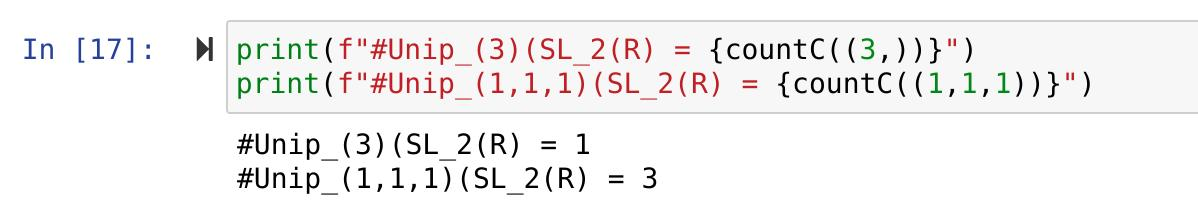
\includegraphics[width=\textwidth]{SL2-unip}
  \end{itemize}
\end{frame}

\begin{frame}{Unitary dual}
     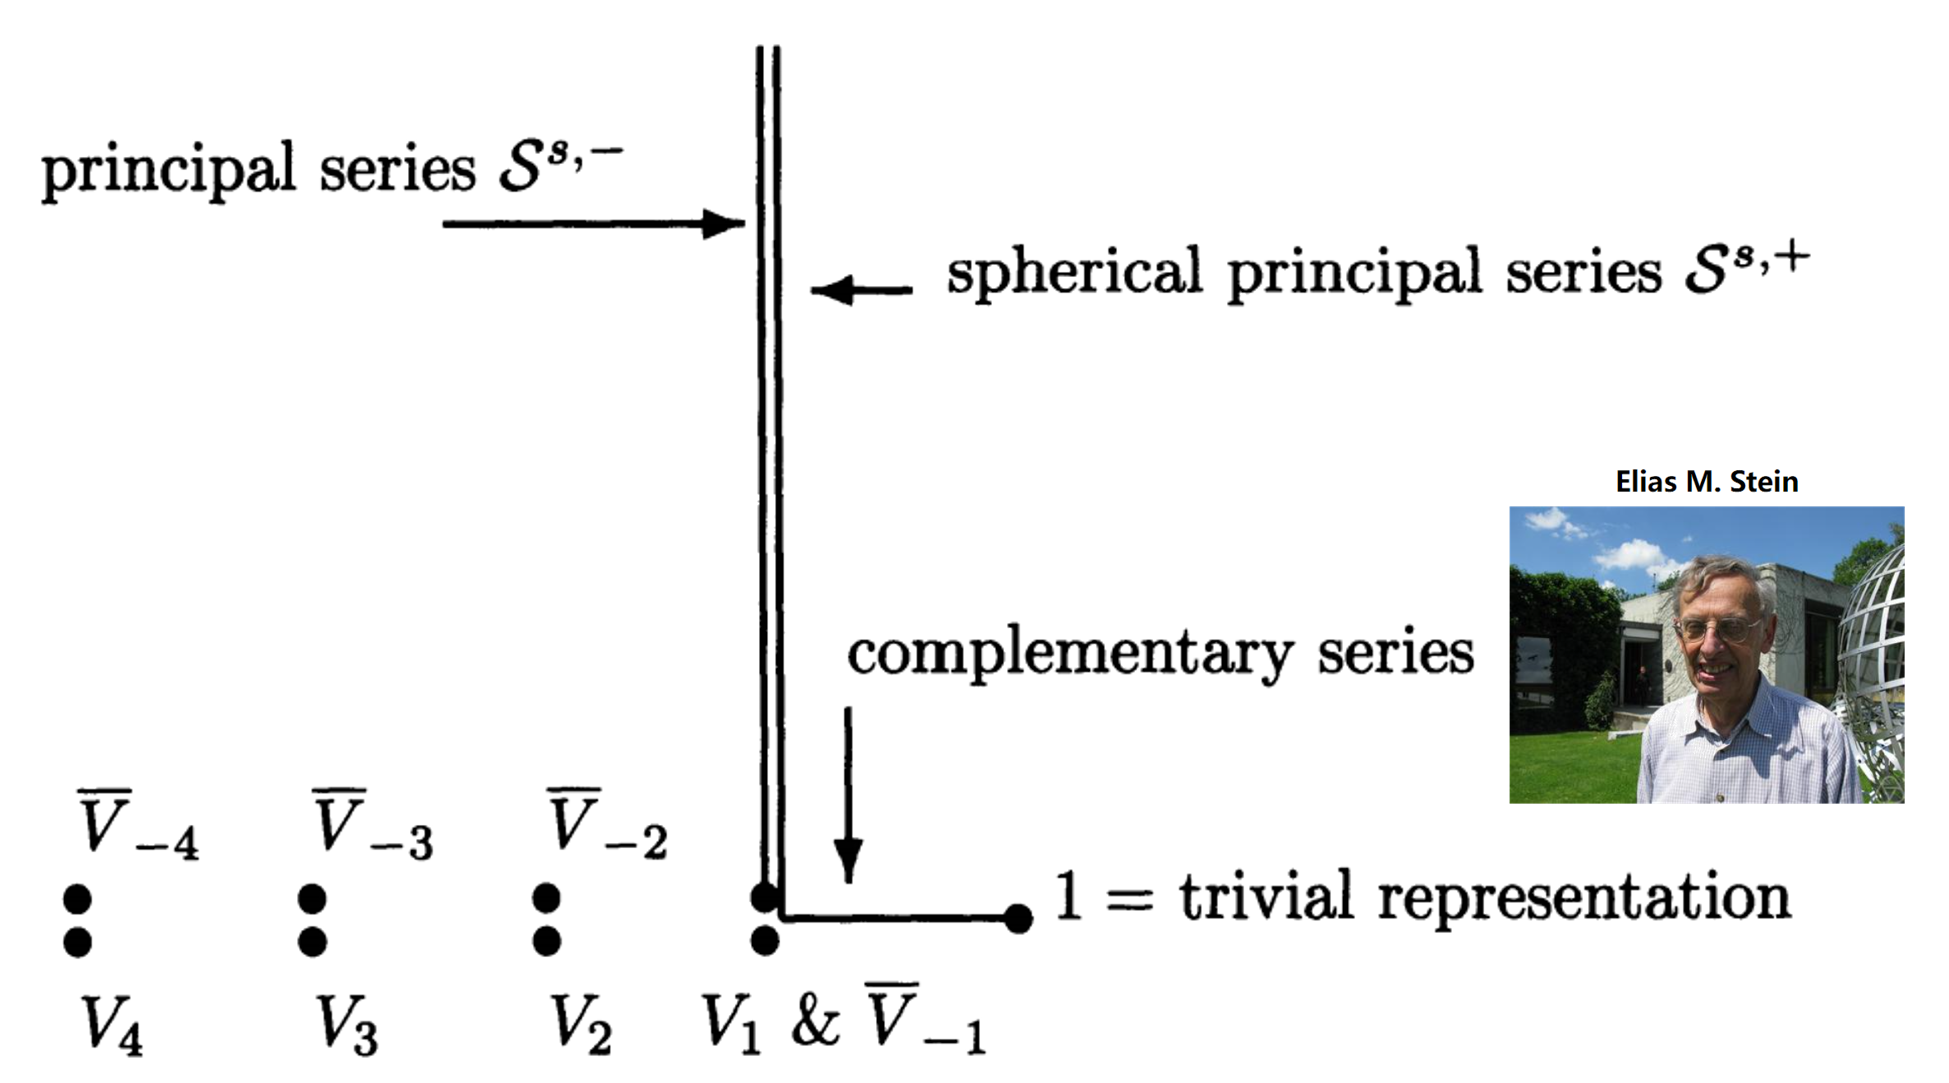
\includegraphics[width=\textwidth]{unitary_sl2}
\end{frame}

\begin{frame}{Complex associated variety}
  \begin{itemize}
    \item $\pi \in \Unip_{\ckcO}(G)$
    \item[] $\Longleftrightarrow$ $\pi$ has inf. char.
          $\lambda_{\ckcO}$ and $\AV_\bC(\pi) = \overline{\cO}$
          \item $\Nil(G_\bC)\ni \cO $
          \item[] $:=$ the Lusztig-Spaltenstein-Barbasch-Vogan dual of $\ckcO$.
    \item[] $\cO$ is a \emph{special nilpotent orbit.}
    \item \emph{Question: } For $\cO \in \Nil(G_{\bC})$, inf. char. $\lambda$,
    $\# \set{\pi \in \Irr(G) : \text{inf. char. $\pi=\lambda$ and
      } \AV_{\bC}(G) = \overline{\cO}} {\color{red}= ??}$.
    \item This is question also relevent if one consider non-special unipotent
    representations (defined by Losev, Mason-Brown, and Matvieievskyi).
  \end{itemize}
\end{frame}

\begin{frame}{Counting irr. repn. with a fixed asso. variety\\ (integral case)}
  \begin{itemize}
    \item \emph{Assume:} inf. char. $\lambda$ is integral.
    \item[] {\color{purple} Fact}: $\AV(\text{prim. ideal w. inf. char.
          $\lambda$})=\overline{\text{a special nilpotent orbit}}$
          \pause
    \item[] Double cell $\cD$ in $\Irr(W)$ $\longleftrightarrow$
          the special nilpotent orbit $\cO$.
    \item $\Coh_{[\lambda]}(G)$: the coherent continuation repn. based on
          $\lambda+X^{*}$. \pause
    \item $W_{\lambda}:=\set{w\in W | w \lambda = \lambda}$
    \item[] \emph{ Theorem: } \only<4->{If $E_{8}$ is not a simple factor of
          $G$, then}
          \[
          \begin{split}
            & \set{\pi \in \Irr(G) |\text{inf. char. }=\lambda,  \AV_\bC(\pi) = \overline{\cO}}\\
            &= \sum_{\tau\in \cD} [\tau:1_{W_\lambda}]_{W_{\lambda}} \cdot [\tau: \Coh_{[\lambda]}(G)]
          \end{split}
          \]
    \item[]
  \end{itemize}
\end{frame}

\begin{frame}{Counting unipotent representations}
  \begin{itemize}
    \item Complex reductive groups (Barbasch-Vogan)
    \item[] $\# \Unip_{\ckcO}(G) = \#$ Lusztig's canonical quotient. \pause
    \item $\U(p,q)$
    \item[] $\# \Unip_{\ckcO}(G)= \#$ real forms of its BV-dual $\cO$. \pause
    \item $\SU(p,q)$, restriction from that of $\U(p,q)$ or the double cover of $\U(p,q)$.
    \item Real classical groups
    \item[] $\# \Unip_{\ckcO}(G)= $ painted bi-partitions (BMSZ). \pause
    \item[] \only<7->{{\color{purple} Construction: theta correspondence}}
    \item Spin group
    \item[] very few genuine special unipotent representations. \pause
    \item Exceptional group
    \item[] Atlas of Lie group
  \end{itemize}
\end{frame}


\begin{frame}{Dual pairs over finite fields}
  \begin{itemize}
    \item $F:= \bF_q$ a finite field, s.t. $\abs{F} = q$.
    \item $(V,V')$: a dual pair of Hermitian spaces\\
          \begin{tabular}{c|c|c|c}
            \hline
            & $G = \rU(V)$ & $G' = \rU(V')$ &  \\
            \hline
            \hline
            $(A)$ & unitary gp. & unitary gp. &  \\
            \hline
            $(B)$ & odd orthogonal gp. & ``metaplectic'' gp. &  \\
            $(D)$ & even orthogonal  gp. & symplectic gp. &  $p\neq 2$  \\
            $(C)$ &  symplectic gp. & even orthogonal gp.  &   \\
            $(\wtC)$ & ``metaplectic'' gp. & odd orthogonal gp. & \\
            \hline
          \end{tabular}
          \pause
    \item We focus on case $(C)$ today.
  \end{itemize}
\end{frame}




\begin{frame}{Theta lifting/Howe correspondence}
  \begin{itemize}
    \item $V$ symplectic space, $V'$ quadratic space.
    %\item $\rU(V)\times \rU(V')\longrightarrow \rU(V\otimes_F V')$
    \item (modified) Weil representation
          \[
          \omega_{V,V'}:=
            \left(\bbone \boxtimes (\xi\circ {\det}_{V'})^{\half\dim_F V} \right)\otimes
            \omega_{\psi, V\otimes_F V'}
          \]
    \item[] ($\omega_{\psi, V\otimes_{F} V'}$: Weil representation of
          $\rU(V\otimes_F V')$ a la  G\'erardin,\\
          \ \ $\xi$ the quadratic character of $ F^\times$)
    \item[]
    \item Orthogonal gp. acts \emph{geometrically} on the Schr\"odinger model.
    \item Compatible with the \emph{conservation relation}.
  \end{itemize}
\end{frame}

\begin{frame}{Theta lift functor}
  \begin{itemize}
    \item[] \emph{Theta lift functor} %($\cK(\_)$ the Grothendieck group)
          \[
          \begin{array}{rcl}
            \Theta_{V,V'} \colon \Rep(G)  & \longrightarrow & \Rep(G')  \\
            \sigma & \mapsto & \left(\omega_{V,V'}\otimes\sigma^{\vee} \right)_{G}
          \end{array}
          \] \pause
    \item[] \hspace{-3em} $\hhgraph{0.12\textwidth}{Srini2}{Srinivasan}$\hspace{-.5em}
 $\hhgraph{0.09\textwidth}{Howe}{Howe}$
$\hhgraph{0.09\textwidth}{Adams}{Adams}$\hspace{-.5em}$\hhgraph{0.1\textwidth}{Moy}{Moy}$
$\hhgraph{0.09\textwidth}{Aubert}{Aubert}$\hspace{-.5em}$\hhgraph{0.09\textwidth}{Michel}{Michel}$\hspace{-.5em}$\hhgraph{0.09\textwidth}{Rouquier}{Rouquier}$
\item[] \hspace{-2em}
$\hhgraph{0.09\textwidth}{Pan}{Pan}$
$\hhgraph{0.09\textwidth}{Liu}{Liu}$\hspace{-.5em}
$\hhgraph{0.09\textwidth}{Wang}{Wang}$
$\hhgraph{0.09\textwidth}{Gurevich}{Gurevich}$
          ...\pause
    \item[]\hspace{-2em}
          $\hhgraph{0.2\textwidth}{Srini-paper}{{\color{blue}Srinivasan, Weil representations of finite classical groups (1979)}}$
  \end{itemize}
\end{frame}

\def\wtcV{{\widetilde{\cV}}}

\begin{frame}{Conservation relation}
  \begin{itemize}
    \item $\cV', \wtcV'$: Witt towers of even dim. quadratic spaces
    \item[] \hfill$\mathrm{disc} (\cV') \neq \mathrm{disc}(\wtcV')$\hfill\ \pause
    \item \emph{First occurrence index} \vspace{-.5em}
          \[
          n_{V,\cV'}(\sigma) := \min \set{\dim V'| \Theta_{V,V'}(\sigma)\neq 0, V'\in \cV' }
          \]\pause
          \vspace{-2em}
          % \item[] Arguments in M{\oe}glin-Vign\'eras-Waldspurger $\Rightarrow$

          % \item[$\bullet$] $\Theta_{V,V'}(\sigma)$ is irreducible and
          % \emph{\phantom{non-}theta-cuspidal} at\phantom{fer} first
          % occurrence.
          % \item[$\bullet$] $\Theta_{V,V'}(\sigma)$ is irreducible and
          % \emph{non-theta-cuspidal} after first occurrence. \pause
          % \item[] Suppose $\sigma\leftrightarrow \sigma'$ both theta cuspidal.
          % \item $\cE(l,\sigma):= \set{\text{irr. constituent in
          % } \Ind_{P_{l}}^{G_{l}}(\sigma_{l})}$
          %   \item
          %   $\Theta_{V_{l},V'_{l'}} \colon \bZ[\cE(l,\sigma)]\rightarrow \bZ[\cE(l',\sigma')]$
  \begin{block}{Theorem (Conservation relation I)}
    If trivial repn. of $\GL_{1}(\bF_{q})$ is not in the cuspidal support of $\sigma$, then
    \[
      n_{V,\cV'}(\sigma) + n_{V, \wtcV'}(\sigma) = 2\dim V + \delta, \quad \text{with
      }\delta=2
    \]
  \end{block}\pause
  \item Sun-Zhu (2014): $ \delta=\max\set{\text{dim. of an anisotropic quadratic
          space}}$ \pause
  \item Pan (2002):reduction to $p$-adic unip. repn. (cuspidal)
  \item Pan (2022):reduction to the unipotent  case. (general)
  \end{itemize}
\end{frame}



\begin{frame}{Parabolic inductions relevant to $\theta$-correspondence}
  \begin{itemize}
    \item[]\hspace{-3em} {\color{blue}Definition: }$\sigma$ is \emph{theta-cuspidal}
          $\Leftrightarrow$  $\bfone$ of $\GL_{1}(\bF_{q}) \notin $
          cusp. supp. of $\sigma$. \pause
          % \item $V_l$ an $\epsilon$-Hermitian space in the Witt tower of $V$
          % s.t. $\dim V_l = \dim V+2l$.
    \item $V_l = V \oplus \bH^l$ ($\bH$ the hyperbolic space) % when $l\geq 0$.
    % \item $V = V_l \oplus \bH^{-l}$ when $l<0$.
    \item A parabolic subgp. $P_l$ of $G_{l}:=\rU(V_l)$ with Levi \vspace{-.5em}
          \[
          L_l := \underbrace{\GL_1(F)\times \cdots \times \GL_1(F)}_{l\text{-terms}} \times \rU(V)
          \]
          \vspace{-1em}
          \pause
    \item Harish-Chandra series:
          $\cE(l,\sigma)=\Big\{\text{irr. constituents in }
           \Ind_{P_{l}}^{G_{l}}\  \underbrace{\bbone \otimes \cdots \otimes \bbone}_{l\text{-terms}} \otimes \sigma\Big\}$.
          \vspace{-.5em}\pause
          % \[
          %   \sigma_{l} := \underbrace{ \bbone \otimes \cdots \otimes \bbone}_{l\text{-terms}} \otimes \sigma .
          % \]
          \[\footnotesize
          \sigma_{l} :=
          \begin{pmatrix}
            \underbrace{
            \begin{matrix}
              \bfone &     &  \\
                     & \ddots &\\
                     &     & \bfone \\
            \end{matrix}}_{l\times l} & \\
                     & \sigma &  \\
                     &   & \ddots  \\
          \end{pmatrix}
          \]
  \end{itemize}
\end{frame}


\newsavebox{\dk} \savebox{\dk}{ \tikzstyle{vertex}=[circle, draw, minimum
  size=0pt] \newcommand{\vertex}{\node[vertex]}
  \begin{tikzpicture}
    \vertex[label=below:{$s_1$},label={$q$}] (s1) at (-2,0) {};
    \vertex[label=below:{$s_2$},label={$q$}] (s2) at (-1,0) {};
    \vertex[label=below:{$s_{l-2}$},label={$q$}] (s3) at (1,0) {};
    \vertex[label=below:{$s_{l-1}$},label={$q$}] (sl) at (2,0) {};
    \vertex[label=below:{$t_{l}$},label={$q^{\mu}$}] (tl) at (3,0) {}; \draw[]
    (s1) -- (s2); \draw[dashed] (s2) -- (s3); \draw[] (s3) -- (sl);
    \draw[double] (sl) -- (tl);
  \end{tikzpicture}
} \newsavebox{\dkgen} \savebox{\dkgen}{ \tikzstyle{vertex}=[circle, draw,
  minimum size=0pt] \newcommand{\vertex}{\node[vertex]}
  \begin{tikzpicture}
    \vertex[label=below:{$s_1$},label={$\nu$}] (s1) at (-2,0) {};
    \vertex[label=below:{$s_2$},label={$\nu$}] (s2) at (-1,0) {};
    \vertex[label=below:{$s_{l-2}$},label={$\nu$}] (s3) at (1,0) {};
    \vertex[label=below:{$s_{l-1}$},label={$\nu$}] (sl) at (2,0) {};
    \vertex[label=below:{$t_{l}$},label={$\nu^{\mu}$}] (tl) at (3,0) {}; \draw[]
    (s1) -- (s2); \draw[dashed] (s2) -- (s3); \draw[] (s3) -- (sl);
    \draw[double] (sl) -- (tl);
  \end{tikzpicture}
}


\def\Norm{{\mathrm{Norm}}}
\begin{frame}{Hekce algebra
    $\sH_{l,\sigma}:=\End_{G_{l}}(\Ind_{P_{l}}^{G_{l}}\sigma_{l}^{\vee})$} % attached to $\sigma$}
  \pause
  \begin{itemize}
    % \item
           %$ \subset \Set{f : G_{l}\to \End(\sigma_{l})}$
       %   acts (by right composition) on
       %   \[
       %   \Hom_{G_{l}}(\Ind_{P_{l}}^{G_{l}}\sigma_{l}, \omega_{V_l,V'_{l'}}).
       %   \]
    \item Howlett-Lehrer + Lusztig:
    \item[] $\sH_{l,\sigma}\cong $ the Hecke algebra of
          $\sfW_l$ with \emph{unequal} parameters
    \item
    $\Norm_{\rU(V_l)}(L_l)/L_l \cong \sfW_l:=\sfS_l \ltimes \set{\pm 1}^l$.\pause
    \[\usebox{\dk}\]
    \item  $\sH_{l,\sigma} = \braket{T_s | s = s_{1}, \cdots, s_{l-1}, t_{l}}$
    with \emph{Quadratic Relations}
           \[
          \begin{split}
            (T_{s_{i}} +1 )(T_{s_{i}} -  q) &= 0 \quad \forall 1\leq i \leq l-1\\
            (T_{t_{l}} - C_1)(T_{t_{l}} -  C_2) &= 0
                                                  \quad \text{with}\quad  q^{\mu} = - \frac{C_{1}}{C_{2}}
          \end{split} \]
    %  \item $C_{1}, C_{2}$ can be determined by theta lifting of $\sigma$ into the two different Witt tower!
    %  \item $ C_{1}C_{2} = - T_{t_{l}}^{2}(1) = -q^{\blue \dim V+\half \delta} $.
  \end{itemize}
\end{frame}



\begin{frame}{The operator $T_{t_{l}}$}
  \[
    (T_{t_{l}} - C_1)(T_{t_{l}} - C_2) = 0 \quad \text{with}\quad q^{\mu} = -\frac{C_{1}}{C_{2}}
  \]
  \begin{itemize}[<+->]
    \item Let $V'$ and $\wtV'$ be the first occurnce spaces in $\cV'$ and
    $\wtcV'$.
    \item Compute the $T_{l}$-action on
          $\Hom_{G_{l}}(\Ind_{P_{l}}^{G_{l}}\sigma_{l}, \omega_{V_{l},V'})$
    \item[] $C_1 = {\color{purple}\gamma_{V'} } q^{\blue \dim V+\half \delta-\half \dim V'}$
    \item[] $C_2 = {\color{purple}\gamma_{\wtV'}}q^{\blue \dim V+\half \delta-\half \dim \wtV'}$
    \item[] $ C_{1}C_{2} = - T_{t_{l}}^{2}(1) = -q^{\blue \dim V+\half \delta} $ \pause
    \item Compare the \emph{power} $\Rightarrow$ Conservation relation.
  \end{itemize}
\end{frame}


\begin{frame}{generic Hekce algebra}
  \begin{itemize}
    \item  $\sfH_{l,\mu} = \braket{T_s | s = s_{1}, \cdots, s_{l-1}, t_{l}}$
          free over $\bZ[\nu^{\half},\nu^{-\half}]$.
    with \emph{Quadratic Relations}
           \[
          \begin{split}
            (T_{s_{i}} +1 )(T_{s_{i}} -  \nu) &= 0 \quad \forall 1\leq i \leq l-1\\
            (T_{t_{l}} + 1)(T_{t_{l}} -  \nu^{\mu}) &= 0
          \end{split} \]
    %  \item $C_{1}, C_{2}$ can be determined by theta lifting of $\sigma$ into the two different Witt tower!
    %  \item $ C_{1}C_{2} = - T_{t_{l}}^{2}(1) = -q^{\blue \dim V+\half \delta} $.
  \end{itemize}
\end{frame}

\begin{frame}{Hecke bimodule and its deformation}
  \begin{itemize}
    \item[] \emph{Assume} theta-cuspidal
          $\sigma\stackrel{\Theta}{\longleftrightarrow}\sigma'$, \pause
    \item Consider the $\cH_{l,\sigma}\times \cH_{l',\sigma'}$-module:
          $\cM:= \Hom_{G_l\times G'_{l'}}(\Ind_{P_{l}}^{G_{l}}\sigma_l\otimes \Ind_{P'_{l'}}^{G'_{l'}}\sigma'_{l'}, \omega_{V_l,V'_{l'}})$ \pause
%    \item Replace $q$ by indeterminate $\nu \leadsto $ generic Hecke algebra $\sfH_{l,\mu}$
  \end{itemize}
  $ \hhgraph{0.10\textwidth}{Tits}{Tits deformation}$ \\ %$R = \bZ[\nu^{\half},\nu^{-\half}]$\\
  $\begin{array}{ccccc}
     \sH_{l,\sigma}\times \sH_{l',\sigma'}& \xleftarrow{\nu=q}& \sfH_{l,\mu} \times \sfH_{l',\mu'} & \xrightarrow{\nu=1}&\bC[\sfW_{l}\times \sfW_{l'}]\pause\\
     \Downarrow & & \Downarrow & & \Downarrow\\
     \Rep_{\bC}(\sH_{l,\sigma}\times \sH_{l',\sigma'})\hspace{-1em} & \xleftarrow{ \ \ \ } &\hspace{-1em} \Rep_{R}(\sfH_{l,\mu}\times\sfH_{l',\mu'})\hspace{-1em} & \xrightarrow{\ \ }& \hspace{-1em}\Rep_{\bC}(\sfW_{l}\times\sfW_{l'})\\
   \end{array}
   $
 \end{frame}

\begin{frame}{Main Theorem (assume $\sigma\stackrel{\Theta}{\longleftrightarrow}\sigma'$ and theta-cuspidal)}

  \begin{block}{Theorem (M.-Qiu-Zou)}
    There is an $\sfH_{l,\mu}\times \sfH_{l',\mu'}$-module $\sfM$ (constructed explicitly)\\
    such that
    \begin{itemize}
      \item
            $\sfM \otimes_{R}\bC_{q} \cong \cM:=\Hom_{G_l\times G'_{l'}}(\Ind_{P_{l}}^{G_{l}}\sigma_l\otimes \Ind_{P'_{l'}}^{G'_{l'}}\sigma'_{l'}, \omega_{V_l,V'_{l'}})$ % \Hom_{P_l\times P'_{l'}}(\sigma_l\otimes \sigma'_{l'}, \omega_{V_l,V'_{l'}}) $
      \item $\sfM\otimes_{R}\bC_{1}$
      % $\vspace{-1em}
      % \[
            $ \cong \displaystyle\sum_{k=0}^{\min\set{l,l'}} \Ind_{\sfW_{l-k}\times \triangle \sfW_{k}\times \sfW_{l'-k}}^{\ \ \ \ \sfW_{l}\ \ \times\ \ \sfW_{l'}} \bfone_{l-k} \boxtimes \varepsilon_{k}\boxtimes\bfone_{l'-k}. $
            % \]
            % \vspace{-1em}
    \end{itemize}
  \end{block}
  \begin{itemize}
    % \item Lusztig/AMR's normalization: $\mu(\sigma),\mu(\sigma') \geq 0$
    \item Theorem + Adams-Moy $\Rightarrow$ Aubert-Michel-Rouquier + Pan \pause
    \item Theorem  $\Rightarrow$ General form of the conservation relation. \pause
    \item[]
    \item When $\mu=1$, $\sfM$ has a geometric realization.
  \end{itemize}
\end{frame}



\begin{frame}{Determine the correspondence between cuspidal repns.}
  \begin{itemize}
    \item Lusztig's map
          $\cE(G,s)\longrightarrow \cE(G^{*}_{s},1)$.
    \item Unipotent cuspidal repn are rare. \pause
    \item Assume: $\cE(G,s) \ni\sigma\leftrightarrow \sigma'\in \cE(G,s')$ is
          cuspidal.
    \item $\tau_{t}$ is cuspdial $\GL_{k}$ repn ($k\neq 1$ or $t\neq 1$).
    \item Consider
          $\cH_{\tau,\sigma}:= \End(\Ind_{(\GL_{k}\times G)U}^{G_{k}} \tau \otimes \sigma)$. \pause
    \item \emph{Lemma}: $\cH_{\tau,\sigma}\cong \cH_{\tau,\sigma'}$.\pause
    \item The lemma+conservation relation $\leadsto$ description of theta
          correspondences between cuspidal repns.
    \item[]
    \item Similar lemma holds in $p$-adic case.
  \end{itemize}
\end{frame}

%\pagestyle{empty}
\begin{frame}{Theta and Hecke algebra / $\bR$?}
  \ \vspace{5em}
  \begin{center}
    \Huge Thank you for listening!
  \end{center}
\end{frame}


\def\VV{{\mathbb{V}}}
\def\tcNV{{\widetilde\cN}_\VV}
\def\tcN{{\widetilde{\cN}}}
\def\Flag{{\mathrm{Fl}}}




\end{document}






        \begin{frame}{Parabolic inductions irrelevant to $\theta$-corr. }
          \begin{itemize}
            \item \emph{3nd Goal: }
            \item[] Determine the theta correspondence between
                  theta-cuspidals.\pause

            \item A parabolic subgp. $P_{r,l}$ of
                  $G_{rl}:=\rU(V\oplus \bH^{rl})$ with Levi \vspace{-.5em}
                  \[
                  L_{l,r} = \underbrace{\GL_r(F)\times \cdots \times \GL_r(F)}_{l\text{-terms}} \times \rU(V)
                  \]
                  \vspace{-1.5em}\pause
                  \[\sigma_{l,\tau} := \underbrace{ \tau \otimes \cdots \otimes \tau}_{l\text{-terms}} \otimes \sigma .
                  \]
                  \pause
            \item Let $\tau\in \Cusp(\GL_{r}(F))$ and $\sigma\in \Rep(\rU(V))$.
                  \[
                  \cE(l,\tau,\sigma)=\set{\text{irr. consist. in
                  } \Ind_{P_{rl}}^{G_{rl}} \sigma_{l,\tau}}.
                  \]
          \end{itemize}
        \end{frame}


        \begin{frame}{Isomorphism of Hecke-algebra. }
          \begin{itemize}
            \item $\tau$ and $\sigma$ irrelevant $\Leftrightarrow$
                  $\tau\neq 1_{\GL_{1}(F)}$ and
                  $\sigma\notin \cE(l,\tau,\sigma'')$ for some $l>0$.
            \item Consider
                  \[
                  \cH_{l,\tau,\sigma}^{op} := \End_{G_{rl}}(\Ind_{P_{l,r}}^{G_{rl}}\tau\otimes \cdots \otimes \tau\otimes \sigma).
                  \]
            \item Suppose $\sigma\stackrel{\Theta}{\longleftrightarrow}\sigma'$
                  and irrelevant to $\tau$.
            \item Kudla + Fourier transform implies:
                  \[
                  \cH_{l,\tau,\sigma} \cong \cH_{l,\tau,\sigma'}^{op} \quad \text{(canonically).}
                  \]
            \item[] $\Rightarrow$
                  $\cE(l,\tau,\sigma)\stackrel{\theta}{\longleftrightarrow} \cE(l,\tau,\sigma')$.\pause
            \item \emph{3nd subGoal: }
            \item[] Determine the theta correspondence between cuspidals.
          \end{itemize}
        \end{frame}

        \def\ch{{\mathrm{ch}}}
        \begin{frame}{Correspondence between cuspdial representations}
          \begin{itemize}
            \item[] Lusztig's maps (endoscopic for finite group of Lie type)
                  \[\Irr(G) = \bigsqcup_{s\in (G^{*})^{\circ}/\text{geo.
                  conj.}} \cE(G,s)\]
            \item
                  $\cE(G,s)\xrightarrow{\ \ \cL\ \ } \cE(G^{*}_{s},1) = \Unip(G^{*}_{s})$
            \item $\cL$ preserve cuspidality.\pause
            \item Let $\tau\in \cE(\GL_{r}(F),t)$ and $\sigma \in \cE(G,s)$
                  cuspidal.
            \item Lusztig: The parameter of $\cH_{l,\tau,\sigma}$ determine
            \item[] \hspace{3em} the multiplicity of $\ch_{t}$ occurs in
                  $\ch_{s}$.
            \item Eg: $\mu(\tau,\sigma)=0 \Rightarrow \ch_{t}$ dose not occur in
                  $\ch_{s}$. \pause
            \item Varying $\tau$, $\mu(\tau,\sigma)$ is sufficient to determine
                  $s$.
            \item $+$ normalization factor $\leadsto$ complete characterization
                  of parametrization + corr. between cuspidal repn.
          \end{itemize}
        \end{frame}


        \pagestyle{empty}
        \begin{frame}{}
          \ \vspace{5em}
          \begin{center}
            \Huge Thank you for listening!
          \end{center}
        \end{frame}
\end{document}


%%% Local Variables: 
%%% coding: utf-8
%%% mode: latex
%%% TeX-engine: xetex
%%% TeX-master: t
%%% End:
